\subsection{Databeskrivelse og databehandling} \label{Sektion: Databeskrivelse}
% god teknik er at lave en label til sektionen, så den er nem at referere til (just in case).


I den følgende sektion vil der blive beskrevet det data der er blevet anvendt i dette projekt. Herudover vil der også blive beskrevet hvordan data er blevet ændret i forhold til det originale data.

I projektet er der blevet anvendt en række geografiske data i dataformaterne vektor og raster samt numeriske data. 

\subsubsection{Digital Terræn Model} \label{Afsnit: Digital Terræn Model}
Modellering og simuleringer af oversvømmelser fra havet kræver en digital terrænmodel (DTM). En DTM er en digital repræsentation af højderne i landskabet i forhold til en reference og adskiller sig fra en Digital Overflademodel (DSM) ved ikke at inkludere bygninger og træer \citep{sdfe_dhm_2020}. En DTM bliver dannet ved brug af LiDAR flyscanning og sker i Danmark over en 5-årig periode. 
I Danmark er det Klimadatastyrelsen (\textit{tidl.} Styrelsen for Digitalisering og Infrastruktur), som står for etableringen af en DTM for hele landet \citep{sdfe_dhm_2020}. \\

I dette projekt er der anvendt en DTM fra 2023. DTM for Danmark er i et GeoTIFF rasterformat med en cellestørrelse på 0,4$\times$0,4m (0,16 m\textsuperscript{2}). DTM for Danmark er i UTM zone 32N projektion og er i ETRS89 koordinatsystem. Den vertikale reference er i DVR90 \citep{sdfe_dhm_2020}. \\
DTM'en anvendt i dette projekt er blevet ændret baseret på størrelsen af hvert studieområde. DTM blev skåret ned til en brugerdefineret afgrænsning af hvert studieområde for at minimere processeringstid. Afgræsningen skete på baggrund af studieområdets topografi og udstrækket af eventuel byzone. Derudover er DTM blevet konverteret til en Digital Hydrologisk Model (DHyM) og bygningspolygoner er blevet brændt ned som ikke passerbare enheder i terrænet. Proceduren for dette er beskrevet henholdsvis i sektion \ref{Sektion: Konvertering af DTM til DHyM} og \ref{Afsnit: Inklusion af bygninger i DHyM}.  


\subsubsection{Arealanvendelses data} \label{Afsnit: Arealanvendelses data}
For at undersøge og kvantificere oktober 2023 stormflodens påvirkning af de udvalgte studieområder, anvendes der et arealanvendelseskort til at beregne og identificere de påvirkede arealanvendelser under stormfloden. \\
Dette blev gjort ved at bruge det danske arealanvendelseskortet BaseMap produceret af \cite{Jepsen_levin_2013}. BaseMap dækker 98\% af Danmarks areal med 35 forskellige arealanvendelsesklasser og er leveret i et rasterformat med en cellestørrelse på 10\times10 m. Kortet er seneset opdateret senest i 2022 med version 4 og det er denne version der er anvendt \citep{levin_basemap04_2022}.\\

For at forsimple visualiseringen af påvirkede arealanvendelser er der blevet udført en reklassifikation af arealklasserne på samme måde som \cite{balstrom_kirby_inundation}. Med denne reklassfikation blev arealanvendelses datasættet trimmet fra 35 oprindelige arealklasser til 13 overordnede klasser. Ved reklassificeringen er en række af klasserne herunder lufthavn, råstofudvinding og Tyskland, som ikke er tilstede i studieområderne, blevet ekskluderet. Klasserne hav, vandløb og søer er også blevet ekskluderet, da de ikke har en relevans for undersøgelsen.\\ Dette resulterer i 8 overordnede klasser der er vist i tabel \ref{Tabel: arealanvendelses klasser} samt hvilke klasser fra BaseMap der indgår i de nye aggregerede arealklasser.


\begin{table}[H]
\centering
\renewcommand{\arraystretch}{1.5}
\begin{threeparttable}
\caption{Reklassificerede arealklasser baseret på \cite{balstrom_kirby_inundation} og hvilke arealklasser fra Basemap \citep{Jepsen_levin_2013} der indgår i hver klasse.}
\label{Tabel: arealanvendelses klasser}
\begin{tabular}{@{} l l l @{}} 
\toprule
\textbf{Klasse ID} & \textbf{Aggregerede klasser} & \textbf{BaseMap04 klasser} \\
\midrule
1 & Bebyggede områder &
  \makecell[l]{Bygning, Lav bebyggelse, Lav bebyggelse; Bygning,\\
  Høj bebyggelse, Høj bebyggelse; Bygning,\\
  Bykerne, Bykerne; bygning, Andet bebyggelse,\\
  Andet bebyggelse; Bygning} \\ 
  \addlinespace
2 & Erhverv &
  \makecell[l]{Erhverv, Erhverv; Bygning} \\
  \addlinespace
3 & Rekreativt &
  \makecell[l]{Rekreativt område / sportsanlæg,\\
  Rekreativt område / sportsanlæg; Bygning} \\
  \addlinespace
4 & Infrastruktur &
  \makecell[l]{Vej; befæstet, Vej; ikke befæstet,\\
  Jernbane, Jernbane; Bygning} \\
  \addlinespace
5 & Landbrug &
  \makecell[l]{Landbrug intensivt; midlertidige afgrøder,\\
  Landbrug intensivt; permanente afgrøder,\\
  Landbrug ekstensivt, Landbrug; ikke klassificeret} \\
  \addlinespace
6 & Skov &
  \makecell[l]{Skov, Skov; Våd} \\
  \addlinespace
7 & Naturområde &
  \makecell[l]{Natur; tør, Natur tør; Landbrug ekstensivt,\\
  Natur; våd, Natur våd; Landbrug ekstensivt} \\
  \addlinespace
8 & Uklassificeret &
  \makecell[l]{Ikke kortlagt} \\
\bottomrule
\end{tabular}
\end{threeparttable}
\end{table}




\subsubsection{Hydrologiske tilpasninger} \label{Afsnit: Hydrologiske tilpasninger}
Til konverteringen af DTM til DHyM er der blevet anvendt to hydrologiske tilpasningslag til konverteringen af DTM til en DHyM: Linje- og hesteskotilpasning. Tilpasningerne er begge geometriske dataobjekter defineret af GeoDanmark som polylinjer \citep{GeoDanmark_HydroLag}. \\
Linjetilpasningerne er en defineret som en et-dimensional linjeobjekt, der beskriver en åbning for overfladevands forløb gennem en hindring eller en hindring af overfladevands forløb gennem et terræn \citep{DHMLinje}. 
Linjetilpasningerne er den simpleste hydrologiske tilpasning og forekommer ved bl.a. rør og små vandløb der passerer under veje eller mellem marker. I figur \ref{Subfig: Linjetilpasning} er det et eksempel på en linjetilpasning gennem et rør fra en mark.\\

Hesteskotilpasningerne er defineret af \cite{DHM_Hestesko}, som et hestesko-formet geometrisk objekt der tillader eller begrænser overfladevandets forløb gennem en hindring eller gennem terrænet. Bredden af hesteskoen definerer dermed hindringens størrelse. Hesteskotilpasningerne anvendes ved hindringer i landskabet der er større end et mindre vandløb eller rør og dermed kræver en mere korrekt repræsentation i landskabet. Hesteskotilpasningerne findes især under større broer og tunneller under veje og i figur \ref{Subfig: Hesteskotilpasning} er der vist et eksempel på en hesteskotilpasning fra en cykeltunnel under en vej.
\begin{figure}[H]
    \begin{subfigure}[b]{0.5\textwidth}
        \centering
        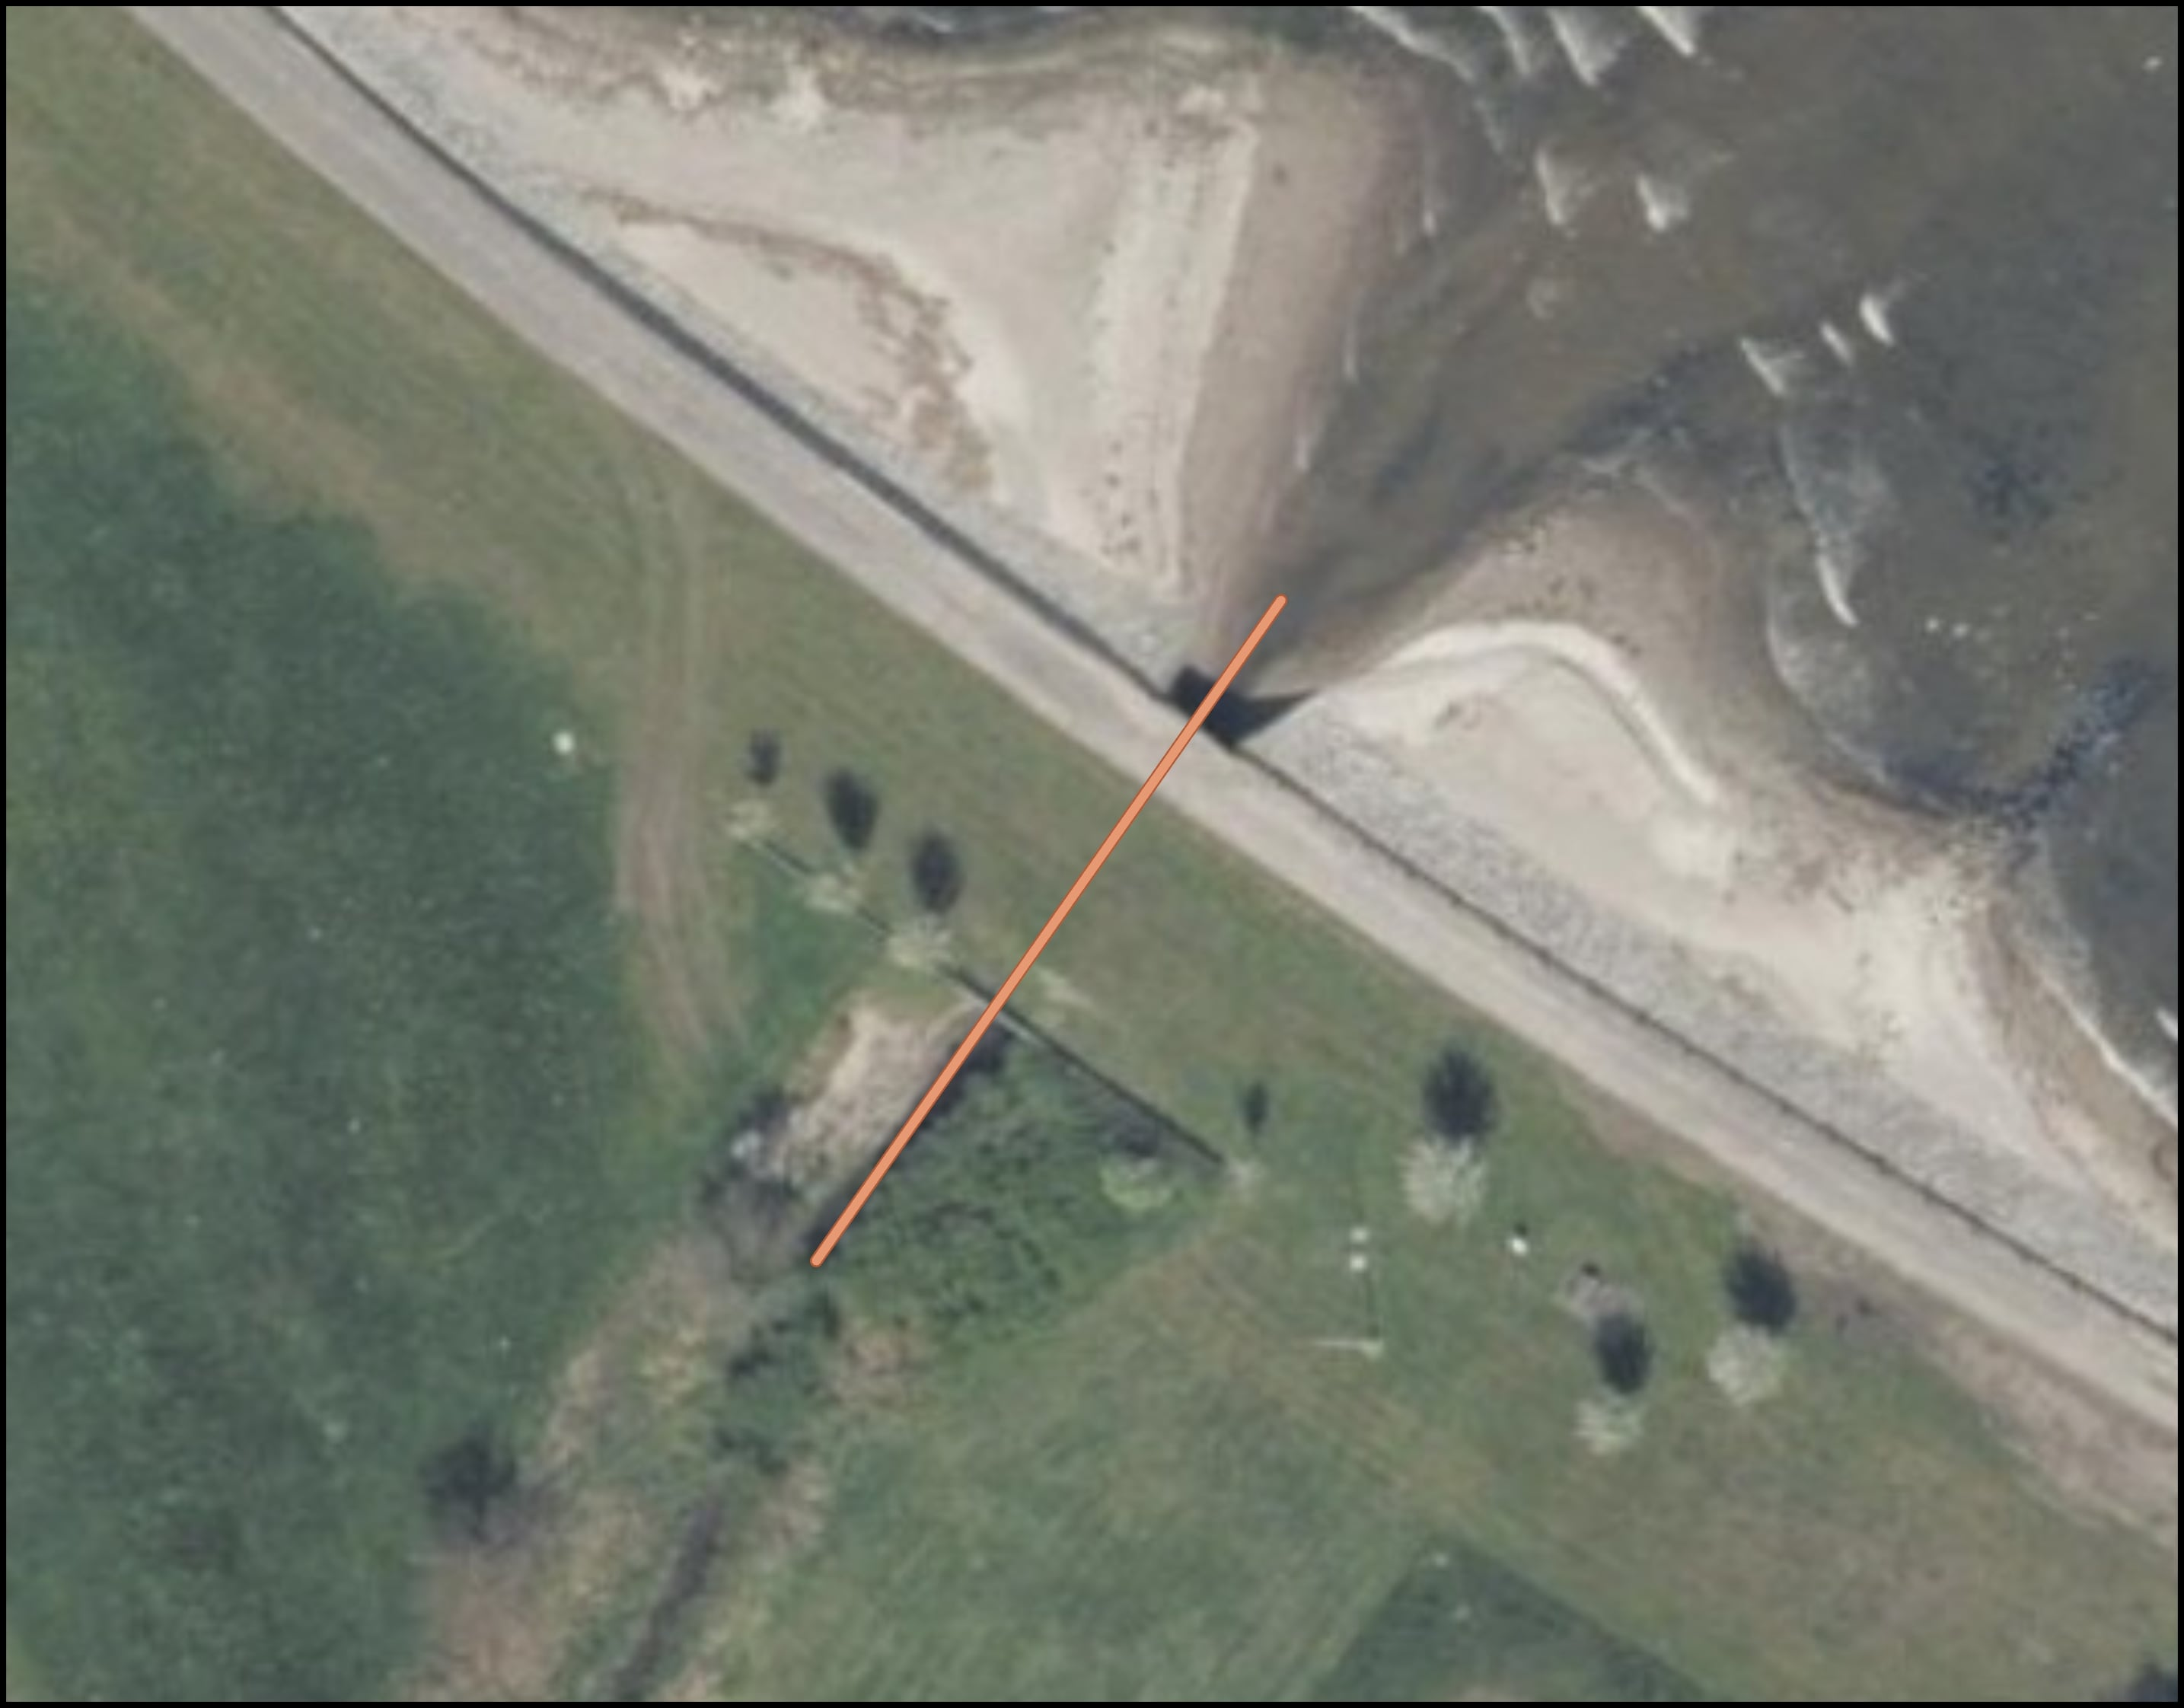
\includegraphics[width=1\linewidth]{images/databeskrivelse/linje.jpg}
        \caption{Linjetilpasning fra et mindre vandløb}
        \label{Subfig: Linjetilpasning}
    \end{subfigure}
    \hspace{0.2cm}
    \begin{subfigure}[b]{0.5\textwidth}
        \centering
        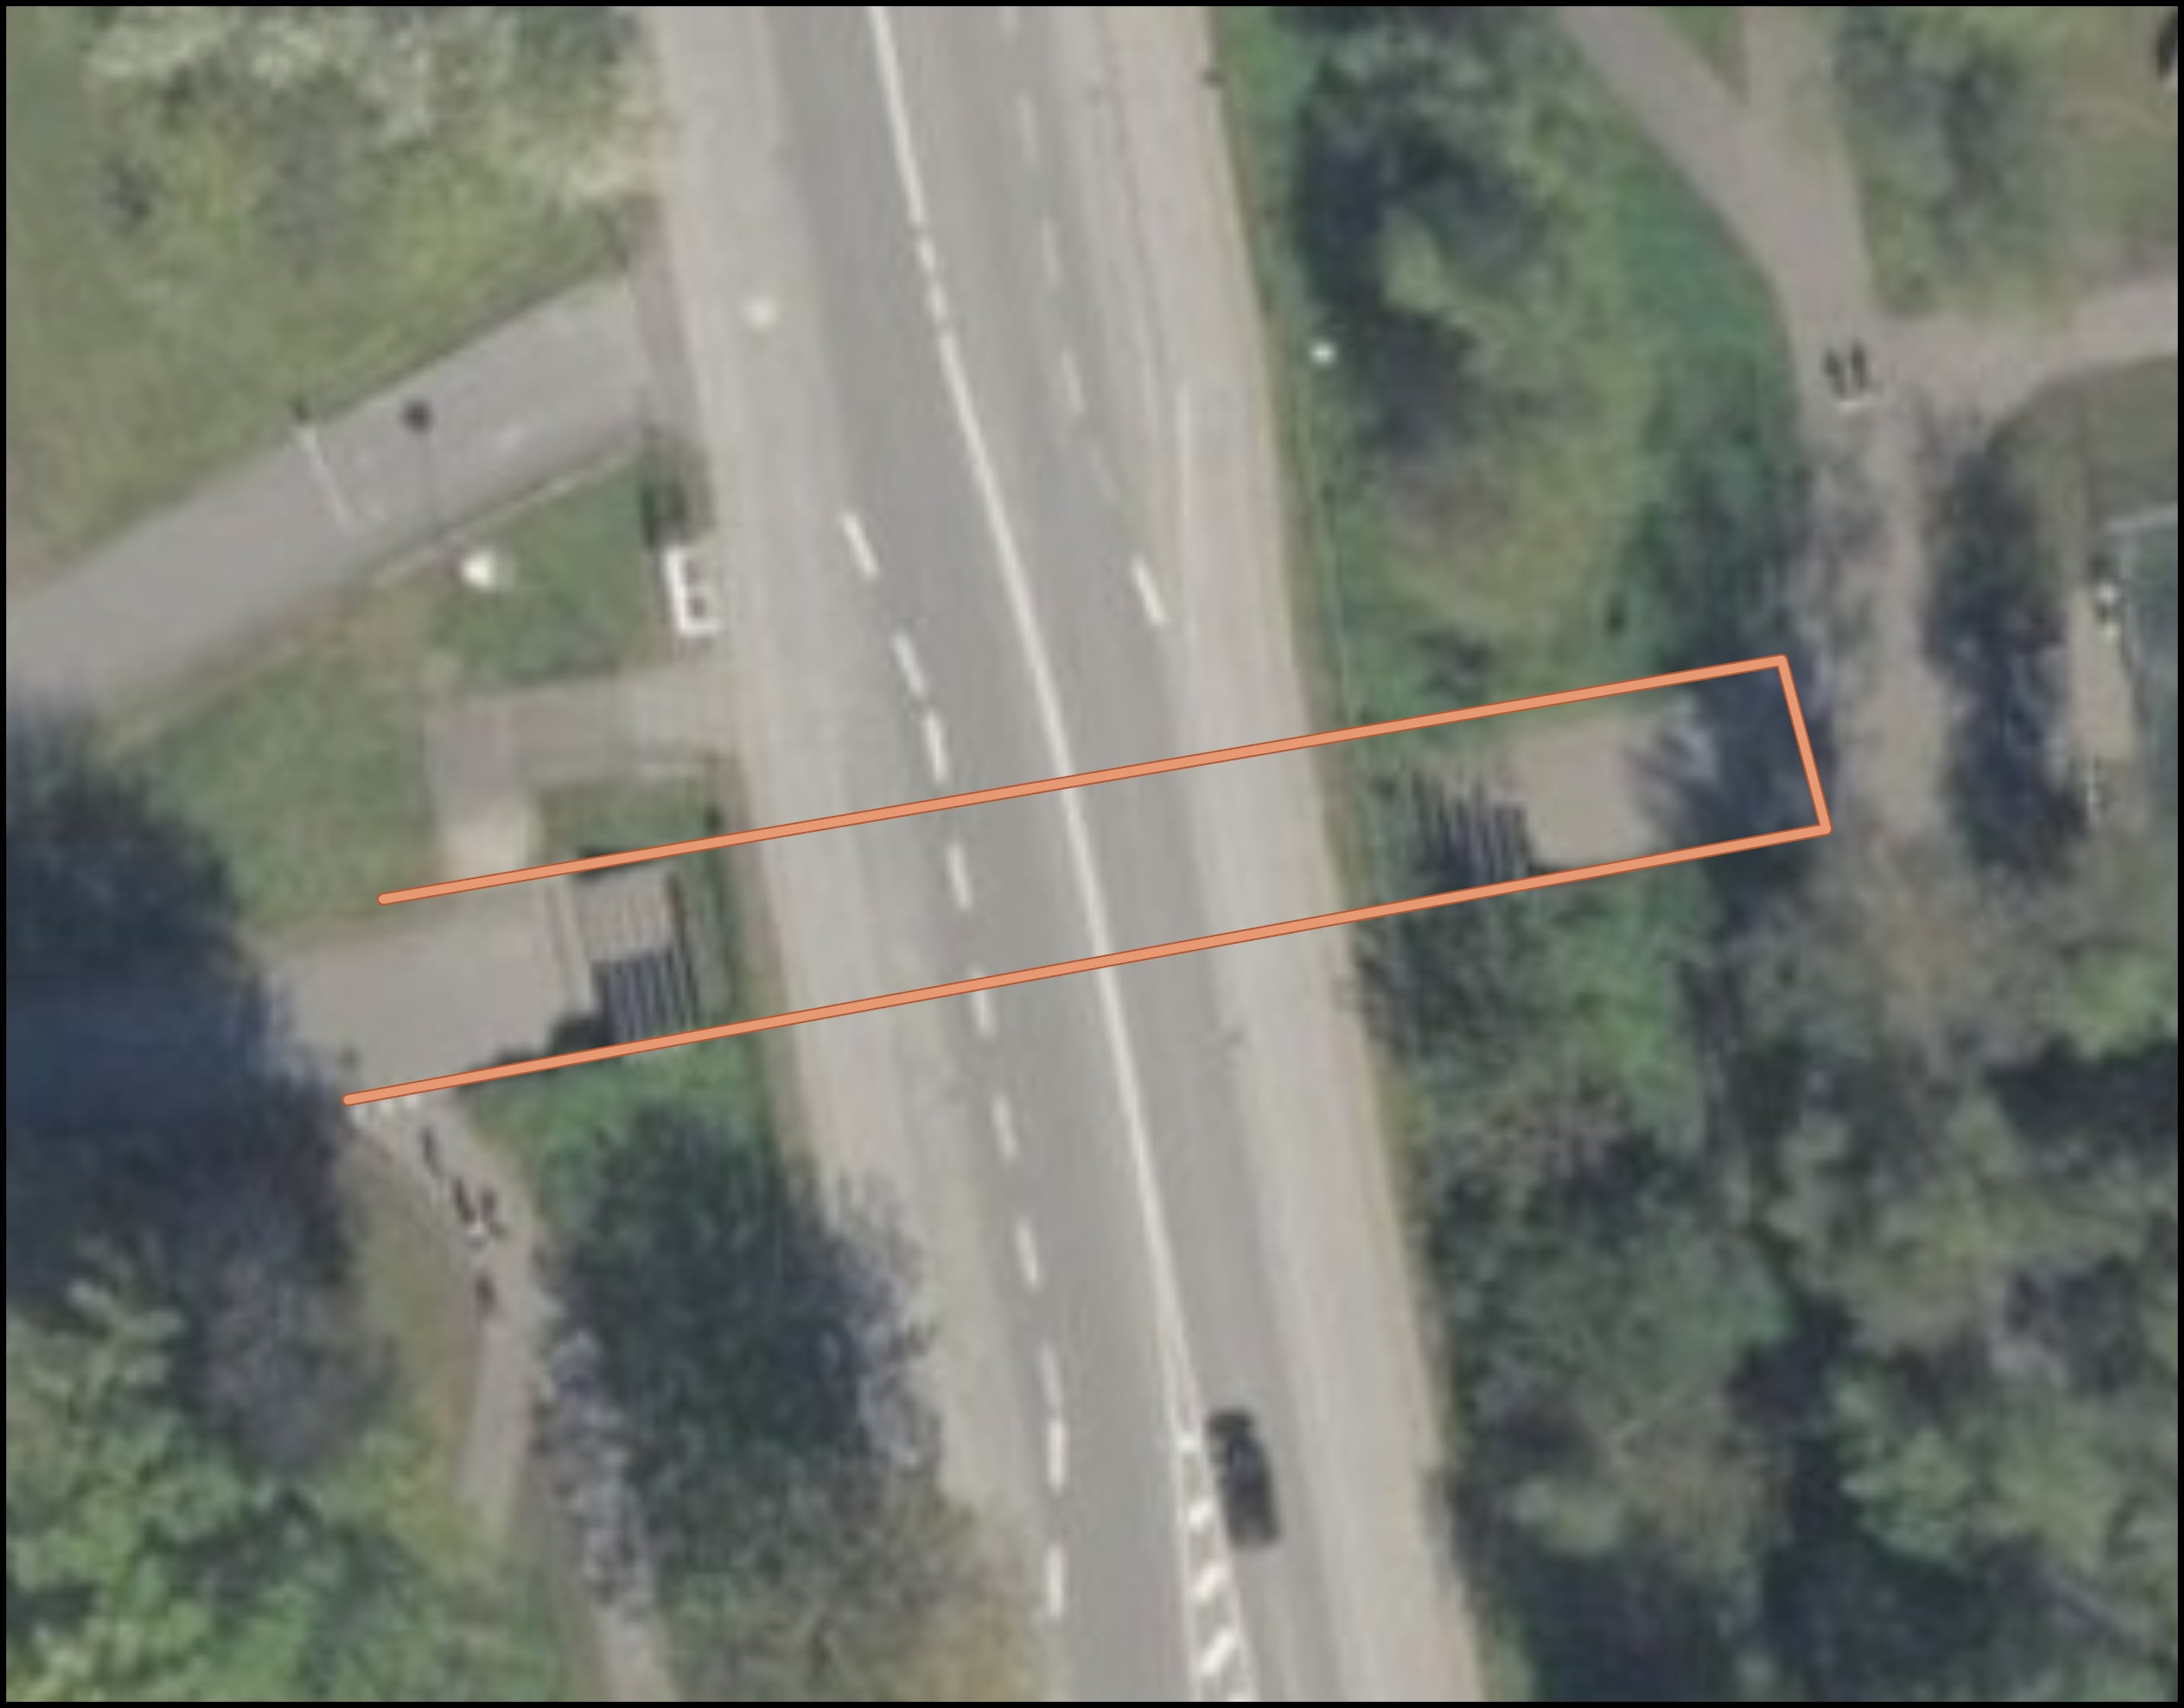
\includegraphics[width=1\linewidth]{images/databeskrivelse/hestesko.jpg}
        \caption{Hesteskotilpasning fra en cykeltunnel under en vej}
        \label{Subfig: Hesteskotilpasning}
    \end{subfigure}
    \caption{Eksempler på hydrologiske linje- og hesteskotilpasninger i Aabenraa}
    \label{Figur: Linje- og hesteskotilpasninger}
\end{figure}

\subsubsection{Vind- og vandstandsdata} \label{Vind- og vandstandsdata}
Til at forstå konteksten bag stormflods hændelsen den 20-21. oktober 2023 er der blevet anvendt vind-og vandstandsdata for måneden oktober 2023. \\
Vinddata er indsamlet fra Danmarks Meteorologiske Instituts (DMI) vejrarkiv \citep{dmi_vejrarkiv} Aabenraa, Guldborgsund og Vordingborg kommune. 
Vinddata er beregnet som gennemsnit for middelvind, højeste 10-min middelvind og den maksimale vindhastighed i m/s for hver dag i måneden. \\

Vandstandsdata er indsamlet på to måder. Data fra Gedser, Hesnæs og Præstø er indsamlet direkte fra DMI's Open Data API-Oceanographic Observation Data ressource \citep{dmi_open_data}. Alt vandstandsdata er optaget hvert 10. minut fra den 1. oktober til den 31. oktober 2023. Data for Præstø er hentet fra Rødvig Havn, ca 25,5 km nordøst, da Præstø ikke har en officiel DMI vandstandsmåler. Dette er den samme station som \cite{cowi_praesto_2025} har anvendt og der tilføjes 30-40 cm som et skøn på vandstanden i Præstø. \\
Data fra Aabenraa Havn er givet direkte fra en samtale med DMI med tilladelse fra virksomheden Aabenraa Havn, da DMI ikke stiller havnens vandstandsmålinger til rådighed for offentligheden. \\

Vandstandsdata fra Gedser Havn havde mange afvigelser, hvor vandstanden svingede fra +200cm til -340cm på 10-min. De datapunkter er fjernet efter et kriterie om at vandstanden ikke vil ændre sig med mere end \pm 25\% på 10 minutter. Hvis vandstanden ikke er indenfor de grænsekriterier, så fjernes datapunktet og det efterfølgende datapunkt tages i betragtning. Hvis det næste datapunkt er indenfor grænsen, så bliver det datapunkt den nye værdi der tjekkes. Den logiske filtrering er vist i ligning \ref{Eq: Outlier vandstand}. Hvor $x$ er et datapunkt i serien og $x_i$ er det næste datapunkt i serien.
\begin{align} \label{Eq: Outlier vandstand}
    \text{Hvis } x_i \in [0.75\times x, 1.25\times x], \text{ så } x \leftarrow x_i \nonumber \\
    \text{Hvis } x_i \notin [0.75\times x, 1.25\times x], \text{ så fjernes } x_i
\end{align}

\subsubsection{Data fra studieområderne og andet anvendt data} \label{Afsnit: Data fra studieområderne og andet anvendt data}
Projektet benytter sig af data modtaget fra de tre kommunerne hvor undersøgelsen finder sted. Den primære data er kommet i form af et raster kort over vandets udbredelse fra stormflodshændelsen i oktober 2023. Alle kortene blev resamplet til en cellestørrelse på 0,4\times0,4m, for at sikre samme cellestørrelse som Inundation modellens resultat. \\
Aabenraa kommune har derudover også givet information omkring beredskabsindsatser, herunder placeringerne af watertubes, og dronebilleder. \\ 


Udover det ovennævnte data er der blevet anvendt en lang række mindre dataprodukter. 
Dette inkluderer et lag med bygningspolygoner der er blevet anvendt til at brænde bygninger ned i DHyM. I sektion \ref{Afsnit: Inklusion af bygninger i DHyM} er der beskrevet hvordan bygningspolygonerne er blevet ændret i forhold til det originale data. En topografisk landpolygon fra \cite{klimadatastyrelsen_landpolygon}, der er anvendt som en maske til Inundation Modellens resultat og vandstandsstignings projektioner fra den sjette \cite{ipcc_report_AR6, NASA_tool} klimarapport, der anvendes til at fremskrive hvordan oktober 2023 stormfloden ville se ud i slutningen af århundredet. 